A de Bruijn sequence (of order $k$), sometimes called a positioning sequence, over an alphabet $\Sigma$, is a sequence of symbols of $\Sigma$ such that all subsequences over $\Sigma$ of length $k$ appear exactly once. This section first explains how to use a graph to represent de Bruijn sequences, and then introduces methods to generate or decode such sequences. Important results on the granddaddy, one of the most interesting de Bruijn sequences, which play a significant role in this work, are also given. 

\subsection{Graph presentation of de Bruijn sequences}

Since the first time introduced in 1946 by de Bruijn himself, the de Bruijn graph and its related sequences have been well-studied and generalized under numerous names, including positioning sequences, m-sequences, shift register sequences \cite{song2021robust,etzion1984algorithms,fredricksen1982survey,lempel1970homomorphism,cohn1977fast}. The goal of de Bruijn was to find a recursive algorithm to enumerate the number of cyclic binary sequences of length $2^k$ such that each binary $k$-tuple appears as a window of length $k$ exactly once in each sequence. 

The first results in the de Bruijn graph focused on the alphabet of size $2$. Later, in 1951, van Aardenne-Ehrenfest and de Bruijn \cite{van1951circuits} generalized the enumeration result for any arbitrary alphabet of finite size $q$, using a generalized graph for an alphabet $\Sigma$ of size $q$. 

\begin{definition}[de Bruijn graph]
    Formally, the de Bruijn Graph of order $k$, $G_{k}$ is a directed graph with $q^{k-1}$ vertices, each one is represented by a word of length $k-1$ over an alphabet $\Sigma$ with $q$ letters. A directed edge from the vertex $\bfx=(x_{0},x_{1},\ldots,x_{k-2})$ to the vertex $\bfy=(y_{1},y_{2},\ldots,y_{k-1})$, represented by the symbol $x_{k}$, where $x_{i},y_{i}\in\Sigma$, if and only if $x_{i}=y_{i}$ for all $1\leq i\leq k-2$. We call this edge $x_{k}$ the out-edge of $\bfx$, and the in-edge of $\bfy$. Progressively, the in-degree and out-degree of a vertex $\bfx$ are the numbers of in-edges and out-edges of $\bfx$ respectively.
\end{definition}  Deduced from the definition, the in-degree and out-degree of each vertex are $q$. Thus, a de Bruijn graph is an Eulerian graph. Figure \ref{fig:dB4} gives an illustration for the graph $G_{4}$.

\begin{figure}[htbp]
    \centering
    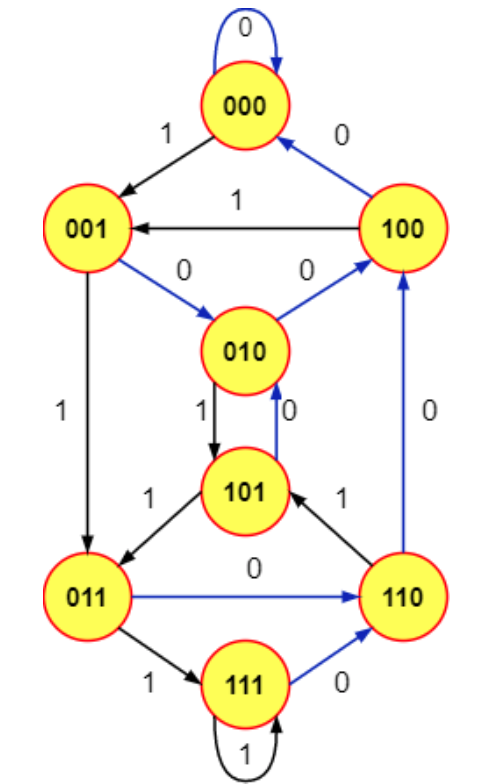
\includegraphics[scale=.3]{fig/dB4.png}
    \caption{de Bruijn graph of order $4$, $G_{4}$.}
    \label{fig:dB4}
\end{figure}

\textbf{Path}: A \textit{path} in the graph is a sequence of edges: $e_{0},e_{1},\ldots,e_{n}$ such that the terminal vertex of edge $e_{i}$ is the the initial vertex of edge $e_{i+1}$ for all $0\leq i\leq n-1$. A \textit{simple path} is a path going through each edge at most one time. Each longest simple path in a de Bruijn graph is an Eulerian cycle. A sequence formed by concatenating the symbol of each edge in the longest simple path in $G_{k}$ is called a (cyclic) de Bruijn sequence of order $k$. All the strings of length $k$ appear exactly once in each such de Bruijn sequence. The acyclic version of the de Bruijn sequence can be obtained by prepending the sequence representing the first vertex in the corresponding Eulerian cycle to the cyclic one. 

\begin{example}
    Consider an Eulerian cycle starting at vertex $000$, then the symbols representing the following edges $0,1,0,1,0,0,1,1,1,0,1,1,0,0,0$ form a de Bruijn sequence order $4$. Adding $000$ to its beginning results in an acylic one: $$0,0,0,0,1,0,1,0,0,1,1,1,0,1,1,0,0,0$$.
\end{example} 

The number of longest simple path in $G_{k}$, and also the number of de Bruijn sequences, have been proved in~\cite{van1951circuits} to be $\dfrac{q!^{q^{k-1}}}{q^{k}}$.
\begin{example}
    For $q=2,\ k=4$, there are $16$ distinct de Bruijn sequences. From figure \ref{fig:dB4}, those de Bruijn sequences are found and listed as follows:   
    \begin{center}
        \begin{tabular}{c c}
            $0000100110101111$ & $0000100111101011$ \\
            $0000101001101111$ & $0000101001111011$ \\
            $0000101100111101$ & $0000101101001111$ \\
            $0000101111001101$ & $0000101111010011$ \\
            $0000110010111101$ & $0000110100101111$ \\
            $0000110101111001$ & $0000110111100101$ \\
            $0000111100101101$ & $0000111101001011$ \\
            $0000111101011001$ & $0000111101100101$ \\
        \end{tabular}
    \end{center}
\end{example}




\subsection{Encode and decode de Bruijn sequences}
Encoding de Bruijn sequences concerns generating an arbitrary de Bruijn sequence or a de Bruijn sequence satisfying some given constraints. Finding a de Bruijn sequence is equivalent to seeking an Eulerian cycle in a de Bruijn graph. In~\cite{fleury1883deux,hierholzer1873moglichkeit}, efficient algorithms to find Eulerian cycles are presented. Especially, the approach in~\cite{fleury1883deux} can be used to generate all binary de Bruijn sequences. However, since the graph must be stored, applying such algorithms to find a positioning sequence requires exponential $O(q^k)$ space.

Besides the graph-based approach, there are other well-known methods to construct such sequences, including \gls{lfsr}, recursive methods, greedy methods, and concatenation approaches.

The idea of \gls{lfsr} is to design a feedback function $f$ mapping length $k$ strings to $\left\{0,1\right\}$. Starting with an initial length $k$ string, $f$ is repeatedly applied to the last $k$ symbols of the current string to generate the next symbol until the maximal length of a de Bruijn sequence is reached. If $f$ is linear, then, the function $F(\alpha)= \alpha f(\alpha)$ is said to be a \gls{lfsr}, where $\alpha$ is a length $k$ string. \gls{lfsr}s based on primitive polynomials generate maximal length sequences (positioning sequences) having length $2^{k}-1$ that miss only the all $0$ string. The downside of this method is that it's compulsory to find a primitive polynomial first.

De Bruijn sequences can also be constructed via recursion by applying Lempel's $D$-morphism $D:\{0,1\}^{m}\to\{0,1\}^{m-1}$ which maps a string $\alpha = \alpha_{1}\alpha_{2}\ldots\alpha_{m}$ to $\beta = \beta_{1}\beta_{2}\ldots\beta_{m-1}$, where each $b_{i} = a_{i} + a_{i+1}\ (mod\ 2)$. Nevertheless, an exponential amount of space is also required by these recursive strategies. 

Surprisingly, greedy approaches are also able to generate de Bruijn sequences. The greedy construction starts with a seed string, then repeatedly applies some greedy rule to determine the next symbol of a sequence. The algorithm stops when it is impossible to add another symbol without creating a duplicate substring of length $k$, or some termination condition is reached. The different explicit greedy rules result in different implementation greedy algorithms~\cite{martin1934problem,alhakim2010simple,fredricksen1982survey,alhakim2021revisiting}. Such constructions, however, have a major drawback: they require exponential space.

Despite many constructions being known, and even a useful survey has been given by Fredricksen~\cite{fredricksen1982survey}, things are not quite the same for the decoding problem. This problem, discovering the position within a particular sequence of any specified $k$-tuple, has been much less well studied. There are just some classical de Bruijn sequences with sub-linear decoding algorithm~\cite{mitchell1996method,tuliani2001bruijn,kociumaka2016efficient}. 

\subsection{Results on lexicographically minimal de Bruijn sequence}

The lexicographically minimal de Bruijn sequence, or \textbf{granddaddy sequence} as called by Knuth~\cite{knuth2013art}, is one the most interesting among other de Bruijn sequences. An example of granddaddy is provided in example~\ref{exp:granddaddy}.
\begin{example}[Granddaddy of order $6$]\label{exp:granddaddy}
    \[0000001000011000101000111001001011001101001111010101110110111111\]    
\end{example}
Both efficient encoder and decoder of this sequence have been found.

The encoding algorithm is actually a concatenation scheme, which is later called \gls{fkm} algorithm, the abbreviation of Fredrickesen, Kessller, and Maiorana, who discovered this strategy~\cite{fredricksen1978necklaces,fredricksen1986algorithm}. Its complexity has been proved to be constant amortized time per symbol by Frank Ruskey et.al~\cite{ruskey1992generating} in 1992.

Though its construction and the related algorithm has been found in 1978, about 40 years ago, the granddaddy's decoder has just been discovered recently in 2016 by Kociumaka, Radoszewski, and W. Rytter~\cite{kociumaka2016efficient}. Denote $\bfx$ as a granddaddy sequence of order $k$, and $v$ is a length $k$ arbitrary substring. Then the decoding algorithm, denoted by $\cD_{KRR}$, returns $\cD_{KRR}(v)$ being the one and only position of $v$ in the whole sequence $\bfx$. Kociumala et.al also proved that $\cD_{KRR}$ works in $O(k^2\log(q))$-time in the word-RAM model and $O(k^{2})$-time in unit-cost RAM model.